\chapter{Stochastic Gradient Descent and Residual Neural Network}

In the previous section, we defined the loss function for knowledge distillation incorporating Rényi divergence. In this chapter, we discuss how to minimize this function using the stochastic gradient descent algorithm. Additionally, we describe the Residual Neural Network architecture, which will be used as a model both for the teacher and the student model in the sequel.

\section{Stochastic Gradient Descent for Knowledge Distillation}

Denote $\mathcal{D}(x,y)$ a joint probability distribution over $\mathcal{X} \times \mathcal{Y}$, where $\mathcal{Y} = \R^n$, and $(x,y) \sim \mathcal{D}$. Let $f_\theta$ be a student model as defined in Definition~\ref{Knowledge Distillation}, with a parameter vector $\theta$. Also denote $f_t$ a pre-trained model, referred to as a teacher. During training the goal is to minimize the loss function with respect to the parameters $\theta$. Our loss function as defined in Equation~(\ref{Rényi Knowledge Distillation}) is given by

\begin{equation}
	\mathcal{L}(\theta,x,y) = (1-\beta) \mathcal{L}_{\text{CE}}(\theta,x,y) + \beta \mathcal{L}_{\alpha}(\theta,x,y),
	\label{Loss function}
\end{equation}
where $\mathcal{L}_{\text{CE}}(\theta,x,y)$ is the cross-entropy loss, $\mathcal{L}_{\alpha}(\theta,x,y)$ is Rényi divergence loss, $\alpha \geq 0$ and $\beta \in (0,1)$.

We define the expected risk of a model $f_\theta$ given a loss function $\mathcal{L}$ as

\begin{equation}
	E(f_\theta) = \E_{(x,y) \sim \mathcal{D}} \left[\mathcal{L}(\theta,x,y)\right],
	\label{Expected risk}
\end{equation}
where the expectation is take with respect to the joint distribution of $(x,y)$.

The expected risk measures the generalization performance of the model $f_\theta$. Unfortunately, the distribution of $(x,y)$ is unknown, thus we approximate the expected risk by the empirical risk for over a given dataset $\mathcal{S} = \{ (x_i, y_i) \sim \mathcal{D}, \, \text{independently for } i = 1, \dots, N\}$, which is defined as

\begin{equation*}
	E_N(f_\theta) = \frac{1}{N} \sum_{i=1}^{N} \mathcal{L}(\theta,x_i,y_i).
\end{equation*}

The gradient descent (GD) algorithm, adopted by \cite{Rumelhart1986} for training neural networks, aims to minimize the empirical risk $E_N(f_\theta)$. After initialization, in each iteration, called an epoch, the parameters $\theta$ are updated using the gradient of the loss function as follows

\begin{equation*}
	\theta_{t+1} = \theta_t - \gamma \frac{1}{N} \sum_{i=1}^{N} \nabla_\theta \mathcal{L}(\theta_t,x_i,y_i),
\end{equation*}
where $\theta_t$ are the parameters of the model after $t$ iterations of the gradient descent algorithm, $\gamma$ is the learning rate and $(x_i,y_i) \in \mathcal{S}$. The number of iterations and learning rate $\gamma$ are hyperparameters. This algorithm is sometimes called the total gradient algorithm. 

A simplification of the previous algorithm is the stochastic gradient descent (SGD) algorithm. In each iteration, the parameters $\theta$ are updated as follows

\begin{equation*}
	\theta_{t+1} = \theta_t - \gamma \nabla_\theta \mathcal{L}(\theta_t,x_t,y_t),
\end{equation*} 
where $(x_t, y_t) \in \mathcal{S}$ denotes a sample drawn from the dataset at iteration $t$.

As noted by \cite{Bottou2010}, SGD directly optimizes the expected risk (\ref{Expected risk}) since the datapoints are randomly drawn from the ground truth distribution.

According to \cite{Bottou1991}, there are few advantages of using SGD over GD. Such as, in datasets with redundancy, only a small subset of datapoints is needed to obtain a good estimate of the gradient, making SGD more efficient. Also, while gradient descent may converge to a local minimum from which it cannot escape, the random effect in SGD often prevents such behavior.

On the other hand, the main drawback of stochastic gradient descent is the high variance of the estimator of the expected risk, as it relies on a singular sample per iteration. To retain the advantages while reducing variance, the mini-batch stochastic gradient descent algorithm can be introduced. In each iteration, a random subset (mini-batch) of $B < N$ data points is sampled from the training dataset $\mathcal{S}$. The algorithm is defined as follows

\begin{equation*}
	\theta_{t+1} = \theta_t - \gamma \frac{1}{B} \sum_{i=1}^{B} \nabla_\theta \mathcal{L}(\theta_t,x_{t_i},y_{t_i}),
\end{equation*}
where $\mathcal{B}_t = \{(x_{t_i},y_{t_i})_{i=1}^B\}$ denotes mini-batch sampled at iteration $t$. Clearly, when $B = 1$, the algorithm reduces to SGD.

Additionally, we introduce weight decay $\lambda$ regularization term to discourage large values of $\theta$, along with Nesterov momentum $\mu$ based on the formula from \cite{Sutskever2013}. Both $\lambda$ and $\mu$ are hyperparameters. The resulting algorithm is as follows

\begin{equation*}
	\begin{aligned}
		b_{t+1} &= \mu b_t + \left( \frac{1}{B} \sum_{i=1}^{B} \nabla_\theta \mathcal{L}(\theta_t,x_{t_i},y_{t_i}) + \lambda \theta_t \right), \\
		\theta_{t+1} &= \theta_t - \gamma \left( \frac{1}{B} \sum_{i=1}^{B} \nabla_\theta \mathcal{L}(\theta_t,x_{t_i},y_{t_i}) + \lambda \theta_t + \mu b_{t+1} \right),
	\end{aligned}
\end{equation*}
where $\mathcal{B}_t = \{(x_i,y_i)_{i=1}^B\}$ denotes mini-batch sampled at iteration $t$.

In practice, an adjustment to this method is used, where in each epoch, the dataset is randomly shuffled and divided into mini-batches of size $B < N$, and each mini-batch is processed sequentially, so that every data point is used once per epoch.

Let $z=f_{\theta_t} (x)$ be the computed logits of the student model. The gradient of the loss function is calculated using backpropagation, that is

\begin{equation*}
	\nabla_\theta \mathcal{L}(\theta_t,x,y) = \frac{\partial \mathcal{L}(\theta_t,x,y)}{\partial \theta} = \frac{\partial \mathcal{L}(\theta_t,x,y)}{\partial z} \frac{\partial z}{\partial \theta},
\end{equation*}
where $z$ is the vector of the logits that the model outputs. From Equations~(\ref{KL gradient}), (\ref{Rényi loss}), (\ref{Rényi gradient}) and (\ref{Loss function}) we get

\begin{equation*}
	\begin{aligned}
		\frac{\partial \mathcal{L}(\theta_t,x,y)}{\partial z} &= (1-\beta) \frac{\partial \mathcal{L}_{\text{CE}}(\theta_t,x,y)}{\partial z} + \beta \frac{\partial \mathcal{L}_{\alpha}(\theta_t,x,y)}{\partial z}, \\
		&=(1-\beta)(Q - y) + \beta \frac{T}{\alpha} \left( Q^T - \frac{(P^T)^\alpha \odot (Q^T)^{1-\alpha}}{\langle (P^T)^\alpha, (Q^T)^{1-\alpha} \rangle} \right),
	\end{aligned}
\end{equation*}
where $P^T$, $Q^T$ and $Q$ are defined as in Definition~\ref{Knowledge Distillation} and $\odot$ denotes the element-wise product, $\langle \cdot, \cdot \rangle$ the scalar product, and $(\cdot)^a$ the element-wise exponentiation. Note that in the cross-entropy part of the equation the temperature scaling is not used. Thus, the gradient used in SGD for knowledge distillation using Rényi divergence loss is given by

\begin{equation*}
	\nabla_\theta \mathcal{L}(\theta_t,x,y) = \left[ (1-\beta)(Q - y) + \beta \frac{T}{\alpha} \left( Q^T - \frac{(P^T)^\alpha \odot (Q^T)^{1-\alpha}}{\langle (P^T)^\alpha, (Q^T)^{1-\alpha} \rangle} \right) \right] \frac{\partial z}{\partial \theta}.
\end{equation*}

What remains to be calculated is $\frac{\partial z}{\partial \theta}$, which depends on the architecture of the student model.

\section{Residual Neural Network}

When using knowledge distillation, we need to define the architectures of both the teacher and student models. In this thesis, we chose to use a Residual Neural Network (ResNet) introduced in \cite{He2016}. This architecture is prominent in computer vision, as it addresses the problems of degradation and vanishing/exploding gradients in deep neural networks.

The architecture of ResNet consists of fully connected layers, convolutional layers, and pooling layers. To understand the fully connected layer, we first define a neuron. Neuron is a function that maps $x \in \R^k$ onto $z \in \R$ as

\begin{equation*}
	z = h ( \sum_{i=1}^{k} w_i x_i + b ),
\end{equation*}
where $w_i$ represents the weight between the $i$-th input and the neuron, $b$ is the bias, and $h$ is the activation function. Commonly used activation functions include the identity function, sigmoid, hyperbolic tangent, and the rectified linear unit (ReLU), defined as

\begin{equation*}
	\text{ReLU}(x) = \max(0,x),
\end{equation*}
which is the activation function used in ResNet. ReLU is primarily used for its simplicity and properties of its derivative (see \cite{Agarap2018}).  

A fully connected layer in a neural network consists of multiple neurons with common activation function operating in parallel, each computing an output $z_j$ based on its own weights and biases. The output of a layer is a vector of all individual neuron outputs, i.e. $z = (z_1,\dots,z_l)$, where $l$ represents the number of neurons in a layer.

To create a multi-layer neural network, the output of one layer is fed as the input to the next. The size of each layer may vary, and we denote the total number of layers by $L$.

Another type of layer is the convolutional layer. Here, the input to the layer is $x \in \R^{h \times w \times c}$, representing an image, where $h$ denotes height, $w$ width and $c$ number of channels. The output is also an image $y$ given by

\begin{equation}
	y_{i,j,k} = \sum_{m = -H}^{H} \sum_{n = -W}^{W} \sum_{l=1}^{c} x_{i+m,j+n,l} \cdot K_{m,n,l,k},
	\label{convolution}
\end{equation}
where $i = 1+H, \dots, h-H$, $j = 1+W, \dots, w-W$, $k=1,\dots,r$, with $r$ being the number of output channels. The $K \in \R^{k_h \times k_q \times c \times r}$ is so-called tensor kernel, where $k_h = 2H+1$ and $k_w=2W+1$. We mostly consider only square kernels, i.e. $k_h=k_w$, usually $k_h=k_w \in \{1,3,5,7\}$.

As we see, the output has a different dimension $y \in \R^{(h-2H) \times (w-2W) \times r}$, compared to the input $x$. This is often undesirable, as we typically want to retain the original height and width of the image. To achieve this, a technique called padding is used. With padding, the output $y$ is computed as in (\ref{convolution}) for all $i=1,\dots,h$ and $j = 1, \dots, w$, while defining $x_{u,v,c} = 0$ for any $u<1$, $u>h$, $v<1$ or $v>w$.

The advantage of convolution is that it focuses on local regions of an image, allowing it to detect patterns such as object edges. Additionally, convolution can recognize the same pattern regardless of its location in the image.

We also introduce stride, the output of a layer is computed as

\begin{equation*}
	y_{i,j,k} = \sum_{m = -H}^{H} \sum_{n = -W}^{W} \sum_{l=1}^{c} x_{s \cdot i+m,s \cdot j+n,l} \cdot K_{m,n,l,k},
\end{equation*}
where $s \in \N$ is a stride. If $s=2$, the output is half the height and width of the input. Thus, $y \in \R^{\frac{h}{2} \times \frac{w}{2} \times r}$, assuming $h$ and $w$ are even.

Another type of layer is the pooling layer, which is similar to a convolutional layer with stride, typically set to 2. However, instead of applying a kernel, it applies a non-linear function to the local region. If the function returns the maximum value, it is called max pooling (MaxPool), if it returns the mean, it is called average pooling (AvgPool). There is also a specific type called global max pooling (GMP), where we take the maximum value over the entire image for each channel. As a result, the output is a vector $\R^c$.

A unique feature of a Residual Neural Network is the residual block. This residual block is composed of a function $\mathcal{F}$ and so-called shortcut, represented by an identity function. The function $\mathcal{F}$ represents multiple layers of the neural network and it the part of residual mapping to be learned. The number of layers in $\mathcal{F}$ may vary, but the authors used two layers. The output of this building block $y$ then follows

\begin{equation}
	y = \text{ReLU} ( \mathcal{F}(x) + x ),
	\label{residual_block_identity}
\end{equation}
where $x$ is the input. This process is depicted in Figure~\ref{fig:residual_block}. If $y$ and $x$ are of a different dimension, we perform linear projection on $x$, thus, we get

\begin{equation}
	y = \text{ReLU} ( \mathcal{F}(x) + W x ),
	\label{residual_block_projection}
\end{equation}
where $W$ is a fixed (non-trainable) projection matrix of appropriate dimensions.

\begin{figure}[h!]
	\centering
	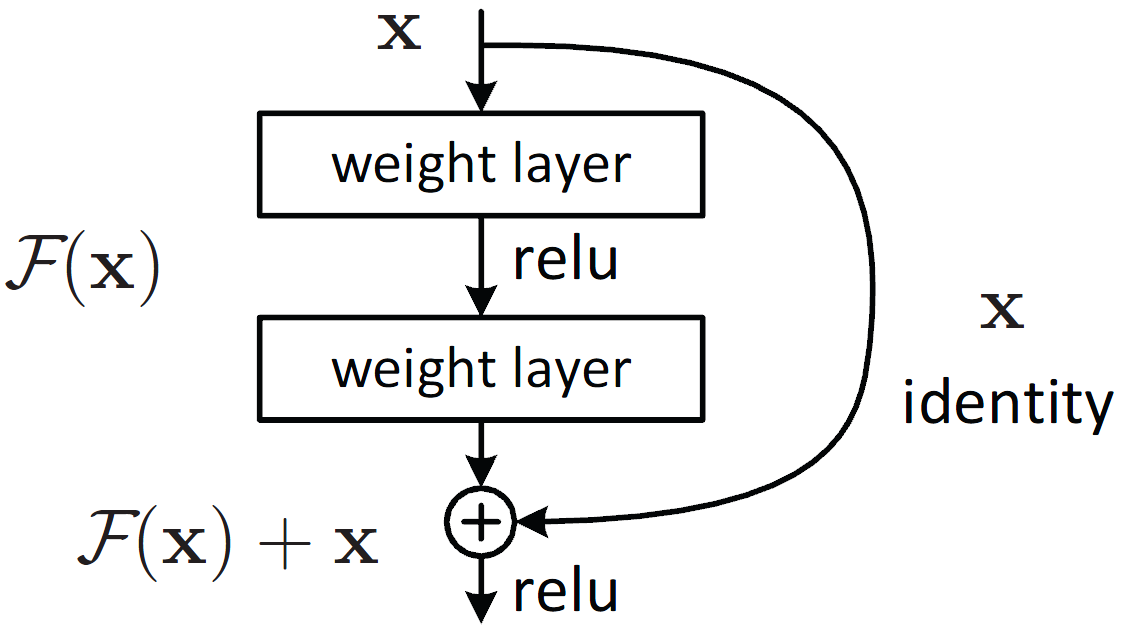
\includegraphics[width=0.44\textwidth]{../img/residual_block.png}
	\caption{Residual block (\cite{He2016}).}
	\label{fig:residual_block}
\end{figure}

The identity mapping helps the gradient propagate more effectively through the neural network, even in deep architectures. It also provides the network with the ability to skip the transformation $\mathcal{F}(x)$ entirely, in cases where the identity mapping is optimal. This also allows the network to learn residuals as small adjustments to the identity function, rather than requiring the network to learn a complete transformation from scratch.

Now, we can define the plain network as described in \cite{He2016}, which serves as the basis for ResNet. The plain network was inspired by VGG nets, which were the state-of-the-art architecture at the time of publication (see \cite{Simonyan2014}). The network starts with a convolutional layer with kernel size $7 \times 7$, continuing with many convolutional layers with kernel size $3 \times 3$. Two design rules are followed. When performing convolution with a stride of 1, the number of kernels matches the number of input channels. However, when using a stride of 2, the number of kernels doubles to preserve the complexity. The network ends with a global average pooling layer and a fully-connected layer. The VGG type network (VGG-19) and the plain network are shown in Figure~\ref{fig:resnet} (left and middle, respectively).

A Residual Neural Network is constructed from the plain network by introducing shortcuts, every two layers, as shown in Figure~\ref{fig:resnet} (right), where solid lines represent the use of Equation~(\ref{residual_block_identity}), and dotted lines represent the use of Equation~(\ref{residual_block_projection}).

There are different variants of ResNet models, distinguished by the number of layers, which affect their capacity and performance. The most commonly used variants are ResNet18, ResNet34, ResNet50, ResNet101, and ResNet152, where the number indicates the total number of layers.

\begin{figure}[h!]
	\centering
	\includegraphics[width=0.6\textwidth]{../img/resnet.png}
	\caption{Example of network architecture (\cite{He2016}). Left: VGG-19 model as a reference. Middle: a plain network with 34 layers. Right: residual network with 34 layers (ResNet34).}
	\label{fig:resnet}
\end{figure}